\documentclass[11pt,twocolumn]{jarticle} %11pt が MS-Word の10.5pt 相当
\usepackage[a4paper,left=23mm,right=23mm,top=27mm,bottom=32mm]{geometry} 

\usepackage[dvipdfmx]{graphicx}
\usepackage{iit-en-sjis} %use iit-en-sjis if the body text is written English.
\usepackage{wrapfig}
\usepackage{algorithm, algpseudocode}
\usepackage{algorithmicx}

\graphicspath{ {imgs/} }

\title{捕食者・獲物環境におけるマルチエージェントの分散型協調学習}
\etitle{Distributed Multi-Agent Cooperation Learning in Predator-Prey Environment}

\author{唐 \ \ 霄}
\eauthor{TANG Xiao}

\advisors{
\footnotesize
\begin{tabular}{ll}
 指導教員: & 延原 肇, 中内 靖, 星野 准一(知能機能工学域)\\
\end{tabular}
}
\eadvisors{
\scriptsize
\begin{tabular}{ll}
Supervised by: & Nobuhara Hajime, Yasushi Nakauchi and Junichi Hoshino (Division of Intelligent Interaction Technologies) \\
\end{tabular}
}

\authorheader{唐 \ 霄}
% use English name when you use the English style

\dateheader{2018年3月}

\abstract{
This paper explains the iit format of master thesis. Standardly, minimum of 8 pages and maximum 24 pages are recommended. If the body text is written in English, English title and English affiliation should come first, then the Japanese. The abstract should be provided in English no matter what language is used in the body text. The data and reference may be included in extra appendix if they can not be included in the body text.. This paper explains the iit format of master thesis. Standardly, minimum of 8 pages and maximum 24 pages are recommended. If the body text is written in English, English title and English affiliation should come first, then the Japanese. The abstract should be provided in English no matter what language is used in the body text. The data and reference may be included in extra appendix if they can not be included in the body text.. This paper explains the iit format of master thesis. Standardly, minimum of 8 pages and maximum 24 pages are recommended. If the body text is written in English, English title and English affiliation should come first, then the Japanese. The abstract should be provided in English no matter what language is used in the body text. The data and reference may be included in extra appendix if they can not be included in the body text.
}

\keywords{keyword-1, keyword-2, keyword-3, keyword-4, keyword-5, keyword-6}

\begin{document}

\maketitle
\thispagestyle{iitheader}
\section{Introduction}
[AI Boom] \par
Recently, AI arouse hot topics around the world, especially the appearence of AlphaGo [reference]. DeepMind introduced their Go player which is called AlphaGo in 2015, they beat several human being's top professional players of over the past two years. And AlphaGo evolved to higher version? which are AlphaGo Master [reference] and AlphaGo Zero [reference]. Not only the application to traditional sports, Game is also a big area which study are ongoing. DeepMind and Blizzard released StarCraft II as an AI research environment [reference] to researchers around the world which could help human-being to have a better acknowledge of game strategy.\par

[Application and shortcomings] \par
Deep Reinforcement Learning (DRL) is one of the technologies which support AI development. There are a lot of applications from game playing [reference] to robot controlling [reference]. Also, Google applied Deep Learning to data center coolinng by 40\% electric cost off [reference]. Healthcare and finance are the areas which are being researched and expected to have a greate impact to sociaty. However, despite the fact that DRL is successfully applied to many single-agent domain tasks, there are varianty of applications which are in multi-agent domain. These application needs multiple agents to evolve together resulting in good communication or cooperation. For instance, multi-character controlling in game playing, multi-agent system in delivery system and so on.

[Task]
\begin{figure}[t]
 \begin{center}
  \includegraphics[width=6cm]{imgs/adversary_chasing.png}
  \caption{Adversary Chasing}\label{fig:adversaryChasing}
 \end{center}
\end{figure}

One representative for multi-agent task is Predator-Prey [reference], showed in figure [fig:adversaryChasing]. In above case, there are 
3 predators, 1 prey and 2 landmarks (obstacles) in this map. Predators move with slower speed compared to prey to chase the faster moving prey. For human being, the cooperation strategy of splitting up and surrounding is absolutely easy to understand and learn. Unfortunately, it is difficult for agent to learn. Although Traditional reinforcement learning such as Q-learning [reference], Policy Gradient performs greatly or even over human being in Atari Game [reference], it performs poorly in multi-agent domain. The reason why the successful RL methods using in single-agent domains could not acquire the same result in multi-agent domain is that along with mult-agent self-learning, the environment becomes non-stationary which failed in convergence. \par

[Agenda] \par
In this work, we first introduce several prior work and related researches and why they failed in multi-agent domain. Then we will explain our proposed method - Distributed Multi-Agent Cooperation Algorithm besed on MADDPG algorithm [reference]. Our method includes the multiple workers distributly working on each thread and the learning rate tuning using Proximal Policy Optimization [reference]. \par

Evaluation experiments shows our method performed better than MADDPG and traditional Deep Reinforcement Learning method DDPG. \par

\section{Related Work} 
In this section, we introduce several related researches and discuss why they cannot be applied to multi-agent domain task.
\subsection{Cover-hueristic Algorithm}
As for prior research for solving Predator-Prey, I have proposed a cooperation searching algorithm towards this task. This method is based on map search using cover-heuristic (maxmizing Predator's moving area and minimizing prey's moving area) and accelarate search by map abstraction and refinement. However, this method performs well in small-size maps but poorly in big-size maps, the computational time is depends on the map size. A agent which could be called intelligent should have its own mind like human beings. This kind of AI is able to take actions based one its own policy.\par


\subsection{Multi-Agent Markov Environment}

\begin{figure}[h]
 \begin{center}
  \includegraphics[width=8cm]{imgs/RL.PNG}
  \caption{Reinforcement Learning}
  \label{fig:rl}
 \end{center}
\end{figure}

The interaction between agent and environment is in [fig], environment gets action from agent and return next state and reward to agent.
We extend singl-agent domain interaction to multi-agent setting. \par
A Markvo Environment in multi-agent could be defined: $N$ agents, 
state $S$ which decribes agents' configuration, 
a set of actions $A_1$, $A_2$ ... $A_n$,
a set of observations $O_1$, $O_2$ ... $O_n$ for each agent.
\[ Observation = Env (Agent) \]
For agent $i$, given $\pi_i$ which could output a action Ai when getting observation Oi. which could be displayed as 
\[ A_i = \pi_i (O_i) \]
The Enviroment get $A_1$, $A_2$ ... $A_n$ from each agent, 
then state S tranfer to next state, and agent recieves Ri from enviroment,
\[ S, R = Env (A) \]
\subsection{Deep Q-learning}
Deep Q-learning (DQN) [reference] is the method proposed by DeepMind. It has a much better performance compared with original RL methods. Especially in discrete action space, DQN reached nearly human level in Atari games.
\begin{equation}
L(\theta) = E_{s,a,r,s'}[(Q^*(s, a|\theta) - y)^2],  
\end{equation}
$$where\ y = r + \gamma\max \bar{Q}^*(s', a')$$
However, due to the connection between continous actions, DQN failed to converge and performed poorly in such domains.
\subsection{Deep Deterministic Policy Gradient}
Deep Deterministic Policy Gradient (DDPG) [reference] is based on Deterministic Policy Gradient [reference] and original Policy Gradient [reference] method. 

\begin{figure}[h]
 \begin{center}
  \includegraphics[width=8cm]{imgs/ddpg.PNG}
  \label{fig:ddpg}
 \end{center}
\end{figure}

DDPG can solve continonous action space problem which DQN cannot tackle. It suses actor-critic architecture to handle the problem that original PG cannot update per step.
\subsection{Asynchronous Advantage Actor Critic (A3C)}
A synchronous variant of A3C - Advantage Actor Critic performs better than A3C.
The simplest way to multi-agent coorperation learning is to do leanring independently for each agent. This first attemp is Q-learning which is a classical algorithm in Reinforcement learning, but it does not perform well []. Contrary to value-based method, policy gradient methods for independently learning also performs poorly. This is because each agent's policy changes during the training time then it turns out to a non-stationary environment. \par

!Recent work has focused on learning grounded cooperative communication protocols between agents to solve various tasks [29, 8, 24]. However, these methods are usually only applicable when the communication between agents is carried out over a dedicated, differentiable communication channel.! \par

Our method is ....

\section{Background}

\subsection{Proximal Policy Optimization}
Althoughm Policy gradient methods are foundamental break-through using Deep Neural Network, it is difficult to obstain good result using policy gradient methods because it is extremely sensetive about choosing learning step size. If iteration step size is too small, training will be very slow; if it is too large, training process will be influenced by noise which turns out to a poor performance and over-fitted result. \par
Proximal Policy Optimization is the method which gets inspiration from Trust Region Policy Optimization and does a well trade-off among implementation simplicity, Sample complexity and Tuning difficulty. PPO tries to calculate a update in every iteration step to minimize lost function and ensures a small deviation compared with previous policy when calculating gradient.
\subsection{Multi-Agent DDPG}
This is method proposed by OpenAI in July. \par
1. MADDPG \par
2. Inferring policies of other agents. \par
3. Policy Ensembles
\section{Proposed Methods}
In this section, we introduce our proposed method - Distributed Multi-Agent Cooperation Learning. The method could be split into two part. 

\begin{figure*}[t]
 \begin{center}
  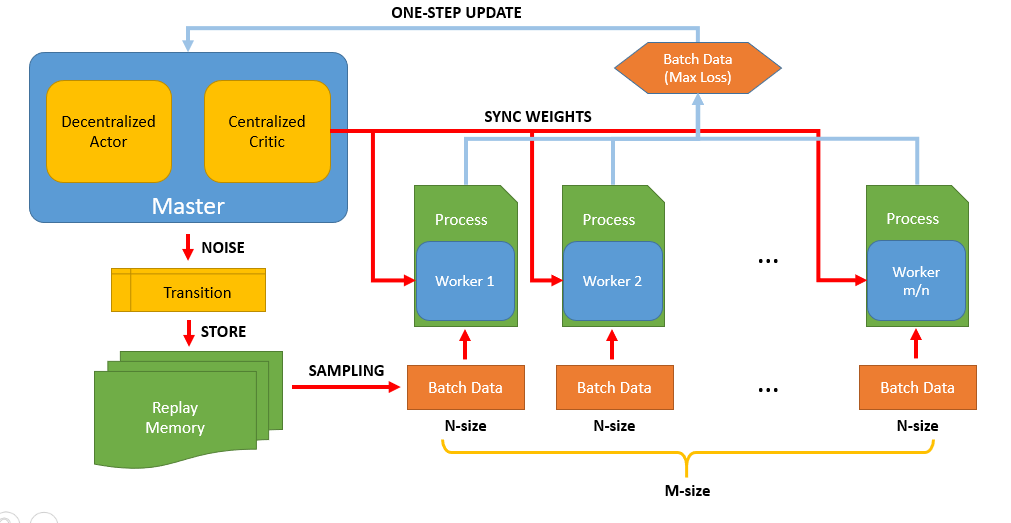
\includegraphics[width=12cm]{imgs/architecture.eps}
  \caption{architecture}
  \label{fig:architecture}
 \end{center}
\end{figure*}

\subsection{Distributed Multi-Agent Cooperation Architecture}
There is brain and several workers in our architecture. Fu We use several workers to work in parallel world to collect batch data with low connectivity. In each worker,  we use brain's policy to choose action, then we give this action (using some noise) to environment and get the batch data (state, actions, rewards, done, next state). And we store this data in to a exchange memory which could accessed by workers (working in each thread). When we have stored batch up to a predifined size, workers stop collecting data from each environment. Meantime, our brain starts to update network using batch data.
\subsection{Leanring Parameter Tuning}
When we are calculating Advantage which could be also called TD-error, by clipping the advantage, we could adjust a proper learning rate for updating actor and critic. This clipping idea comes from clipping suggorate objective in PPO paper. By getting ratio between policy and new policy, we could get the minimal Advantage of ratio and (1-epison, 1+epison), we choose epison = 0.2

\begin{algorithm*}
\caption{Distributed Multi-Agent Cooperation Algorithm}
\begin{algorithmic}
\State {Initiate brain and n workers}
\State {}
\State $New Graph (abstraction level+1)$
\State $Define a queue$
\State {$Initiate\ queue\ with\ head\ node\ pointer\ of\ graph$}
\For {$episode = 1 to M$}
  \State {$Do something$}
\EndFor
\While {$queue \neq empty$}
    \State $node1 \gets queue.pop()$
    \State {$node1\ mark\ as\ "abstracted"$}
    \If {node1 has no unabstracted neighbor}
        \State {Abstract node1 as (level+1) node to new Graph with node1's position}
        \State {$Continue$}
    \EndIf
    \State {$node2 \gets node1's\ unabstracted\ neighbor$}
    \State {Abstract node1, node2 as (level+1) node to new Graph with node1 and node2's average position}
    \State {Push node1, node2's unabstracted neighbor to queue}
\EndWhile
\Return {$new graph$}
\end{algorithmic}
\end{algorithm*}

\section{序論}
執筆要領について述べる。

\subsection{用紙}
A4用紙を縦長に使用する。本文は8ページ(表裏で4枚)以上、24ページ以内を標準とする。

\subsection{ヘッダ・フッタ}
ヘッダの左側には、「筑波大学大学院博士課程システム情報工学研究科修士論文」につづけて、修了年度・月を括弧書きで記述する。
ヘッダの右側には、氏名を記述する。氏名については、見やすくするために適宜空白をいれても差し支えない。

フッタの中央には、ページ番号をハイフンはさんで記述する。

\subsection{1ページ目の体裁}
申請する学位(修士(工学))を四角囲みで記述し、
つづけて修士論文のタイトルをそれぞれ日英表記で記述する。
ただし本文が英文の場合、英日の順に記述する。

つぎに、氏名・所属専攻と指導教員名・指導教員の所属を日英表記で記述する。
氏名・指導教員名については、見やすくするために適宜空白をいれても差し支えない。
ただし本文が英文の場合、英日の順に記述する。


\subsection{要約・キーワード}
修士論文の概要を記述する。
本文が日本語・英語に係らず概要は英語で記述する。


\subsection{本文}
本文は2段組みとし、10.5pで記述する。
句読点は、各分野で用いられる記号を使用する。

\subsection{図表}
論文として印刷に耐えうる品質(解像度)の図表を作成する。
図表中、および、キャプションは、原則として英語を使用する。
キャプションは、図の下と表の上に挿入する。
図番号および表番号は、それぞれ Figure 1、Table 1 のように表記する。
横長の図・表の場合は、段抜きで挿入してもよい。

たとえば、Figure \ref{fig:samplefigure}や Table \ref{tbl:sampletable}を例として示す。

\begin{figure}[t]
 \begin{center}
  \includegraphics{sample.eps}
  \caption{Sample figure}\label{fig:samplefigure}
 \end{center}
\end{figure}

\begin{table}
 \caption{Sample table} \label{tbl:sampletable}
\begin{center}
  \begin{tabular}{c|ccc}
  A & B & C & D\\
  \hline \hline
  a & b & c & d\\
  a & b & c & d\\ \hline
 \end{tabular}
\end{center}
\end{table}

\subsection{数式}
数式のサンプルとして、(\ref{eq:gauss})を示す。
\begin{equation}
 \int _\infty ^\infty e^{-x^2}dx = \sqrt{\pi} \label{eq:gauss}
\end{equation}

\subsection{参考文献}
それぞれの分野の記述法により、十分な数の参考文献を引用する\cite{osamu}。著者が執筆した修士論文に関連する内容の論文等がある場合には、必ず文献として引用する。

\subsection{著者紹介}
学会誌論文の一般的な著者紹介を例に記述する。

\subsection{付録}
本文には書ききれないデータなどは、
付録に収めることができる。付録は、研究室で別途保管する。



\section{\LaTeX スタイルファイルについて}
このサンプルは、筑波大学大学院システム情報工学研究科知能機能システム専攻の修士論文を\LaTeX で作成するためのスタイルファイルである。
配布ファイルは以下の通りである。
\begin{description}
 \item[iit-jp-sjis.sty]  知能機能システム専攻の修士論文のためのスタイルファイル
 \item[templete.tex] スタイルファイルを利用するためのテンプレートファイル
 \item[face.eps] 顔写真用のテスト画像
 \item[sample.eps] Figure のためのテスト画像
\end{description}

スタイルファイルやテンプレートは、適宜改良をして使用してもよい。

\section*{謝辞}
本研究は、・・・・・・深謝する。


%\addcontentsline{toc}{section}{\numberline{}参考文献}

\begin{thebibliography}{9}
\bibitem{osamu}  工学修得, ``修士論文の書き方'', 知能機能システム学会論文誌, Vol.1, No.2, pp.34--56, 2015.
\end{thebibliography}


\vspace{2zh}
\begin{minipage}{73mm}
 \begin{wrapfigure}[6]{l}[-4pt]{30mm} 
 \begin{center}
  \includegraphics[width=30mm]{face.eps}
 \end{center}
 \end{wrapfigure}
 \noindent 筑 \ 波 \ 太 \  郎\\\\
 筑波大学大学院システム情報工学研究科知能機能システム専攻所属
\end{minipage}

\vspace{3zh}
----------------------------------------------\par

\begin{itemize}
 \item Webで公開する論文の概要は、別に作成する。
 \item 修士論文は両面印刷とする。
 \item 修士論文提出時は、ソフトカバーを施して必要部数を大学院教務に提出する。背表紙は不要。
 \item 論文審査後に、両面印刷したもの(綴じていないもの)を専攻長に提出する。
 \item 専攻長は、専攻全員の修士論文をハードカバーにて製本し、専攻室で保管する。
\end{itemize}

\begin{itemize}
 \item Extended summary is also required for uploading onto the web.
 \item The thesis should be printed in double face printing.
 \item Submit your thesis to the academic service office. The thesis should be clapped with a soft-cover.
 \item  Submit your thesis to the chair of the iit, after it has passed the examining meeting. The thesis should not be clapped.
 \item The chair of the iit will bind up all the accepted theses and preserve in his/her office.
\end{itemize}


\end{document}
